% This Source Code Form is subject to the terms of the Mozilla Public
% License, v. 2.0. If a copy of the MPL was not distributed with this
% file, You can obtain one at https://mozilla.org/MPL/2.0/.

\documentclass[a4paper, 12pt]{article}

\usepackage[english, russian]{babel}
\usepackage[T2A]{fontenc}
\usepackage[utf8]{inputenc}
\setlength{\parindent}{1cm}
\usepackage{graphicx}
\usepackage{amsmath}

\begin{document}
	\begin{center}
		\section*{Расчётное задание по теоритической механике: кинематика твёрдого тела}
		\subsubsection*{Выполнил cтудент второго курса Физико-Механического интститута, высшей школы МПУ: Куликовских Илья Михайлович}
		\subsubsection*{группа: 5031503/30001}
		\subsubsection*{Преподаватель: Аюпова Галина Константиновна}
	\end{center}
	
	\textbf{Задача 1.} При поднятии ведра из колодца ускорение ворота диаметром  2.2 см, на который наматывается цепь, изменяется согласно графику на рисунке.
	Определить наибольшую скорость подъема ведра и высоту подъема за
	20 секунд.
	
	\begin{figure}[h!]
		\centering
		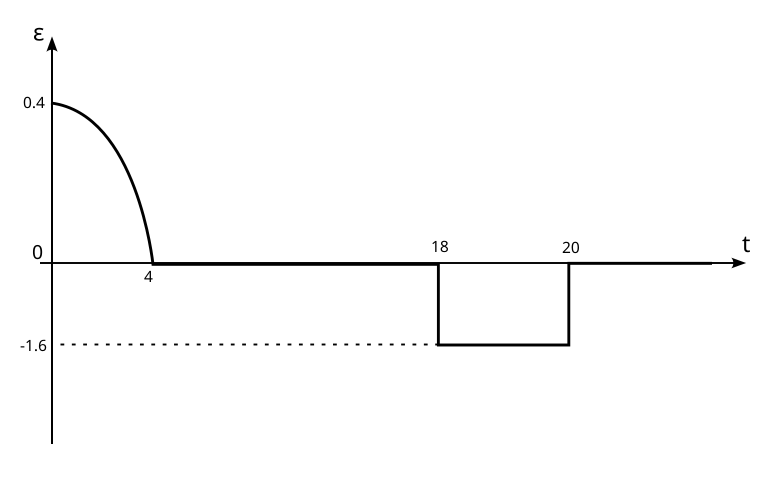
\includegraphics[width=0.8\textwidth]{screenshot001.png}
		\caption{ график функции $\varepsilon = f(t)$}
	\end{figure}
	
	\textbf{Решение: } Определим фунцию $\varepsilon$(t) как кусочно заданую, состоящую из параболы и двух линейных участков. Таким образом получившаяся функция имеет вид:
	
	\begin{center}
		$\varepsilon$(t) = 
		$\begin{cases}
			 -0.025t^2 + 0.4, \forall t \in [0,4] \\
			 -1.6, \forall t \in [18, 20] \\
			 0, \forall t \in (4, 18) \cap (20, + \infty ) \\
		\end{cases}$
	\end{center}
	
	Знает каждый инженер: $\upsilon$ = $\omega$R, а значит для нахождения скорости достаточно найти интеграл $\int\varepsilon(t)dt$ и умножить на радиус.
	\begin{center}
		1)  $\forall t \in [0,4]:  \omega = \int\varepsilon(t)dt = \int(-0.025t^2 + 0.4)dt = -\frac{0.025}{3}t^3 + 0.4t + C$
		
		Н.у. : t=0 $\Rightarrow \omega = 0, следовательно: C = 0$
		
		Скорость на этом участке определяется формулой:
		
		$\upsilon(t) = -\frac{0.025}{3}Rt^3 + 0.4Rt, где R = \frac{d}{2}$ 
	
		2) $\forall t \in [18, 20]: \omega = \int\varepsilon(t)dt = \int(-1.6)dt = -1.6t + C $
		
		Н.у. : t=18 $\Rightarrow \omega = \frac{16}{15}, следовательно: C = \frac{448}{15}$
		
		Скорость на этом участке определяется формулой:
		
		$\upsilon(t) = -1.6Rt + \frac{448}{15}R $
		
		3) $\forall t \in (4, 18) \cap (20, + \infty ): \omega = \int\varepsilon(t)dt = 0 \Rightarrow \omega = 0 \Rightarrow \upsilon(t) = const $
		
		$\upsilon$(t) = 
		$\begin{cases}
			-\frac{0.025}{3}Rt^3 + 0.4Rt, \forall t \in [0,4] \\
			-1.6Rt + \frac{448}{15}R, \forall t \in [18, 20] \\
			const_1, \forall t \in (4, 18) \\
			const_2, \forall t \in (20, + \infty ) \\
		\end{cases}$
		
	\end{center}
	
	Очевидно, что наибольшее значение скорости будет в момент времени $t = 4$, т.к. это крайняя точка промежутка с положительным ускорением. Далее скорость либо не будет менятся, либо будет уменьшаться. 
	
	Тогда:
	\begin{center}		
		$\upsilon_{max} = \upsilon(4) = -\frac{0.025}{3} \cdot 1.1 \cdot 10^{-2} \cdot 64 + 0.4 \cdot 1.1 \cdot 10^{-2} \cdot 4 = 0.012$ (м/с) 
	\end{center}
	
	Теперь найдём значения констант $const_1, const_2$:
	\begin{center}
		$const_1 = -\frac{0.025}{3} \cdot 1.1 \cdot 10^{-2} \cdot 64 + 0.4 \cdot 1.1 \cdot 10^{-2} \cdot 4 = 0.012$ (м/с) 
		
		$const_2 = -1.6 \cdot 1.1 \cdot 10^{-2} \cdot 20 + \frac{448}{15} \cdot 20 = -0.0235$ (м/с)
	\end{center}
	
	Высота подъёма ведра в этом случае определяется выражением:
	\begin{center}		
		
	 	$h(t) = \int_{0}^{20}\upsilon(t)dt = \int_{4}^{0}(-\frac{0.025}{3}Rt^3 + \frac{2}{5}Rt)dt + \int_{4}^{18}0.012dt + \int_{18}^{20}(-\frac{8}{5}Rt + \frac{448}{15})dt = (-\frac{0.025}{12}Rt^4 + \frac{2}{10}Rt^2)\bigg|_{0}^{4} + 0.012t\bigg|_{4}^{18} + (-\frac{8}{10}Rt^2 + \frac{448}{15}Rt)\bigg|_{18}^{20} = (0.0293 - 0) + 0.164 + (3.051 - 3.0624) = 0.182$ (м)
	 	
	\end{center}
	
	\textbf{Задача 2.} Стержень OK, вращаясь вокруг шарнира O с угловой скоростью $\omega$, проталкивает вдоль плоскости OL полудиск радиуса R (рис. б). При этом полудиск все время соприкасается со стержнем вдоль своей кромки ВС. Для	момента, когда угол наклона стержня к плоскости равен $\varphi = 30^\circ$, определите скорости точки A (середины BC) и точки B полудиска. (Считать положительным направлением изменения угла $\varphi$ против часовой стрелки).
	
	
\end{document}